\section{SINATRA}

This thesis centers on being one of the initial development projects of a Cal Poly DSMC code, and implementing of the PIC component to this code. The code-base is code-named SINATRA. SINATRA is developed in C++ for a few purposes. C++ is a current industry standard for large simulations and therefore has a large support base with libraries, a developer community, and a large portion of developers know how to read and develop in C++. It is one of the fastest higher level , object oriented languages.  

\subsection{Object Oriented}

\begin{figure}
    \centering
    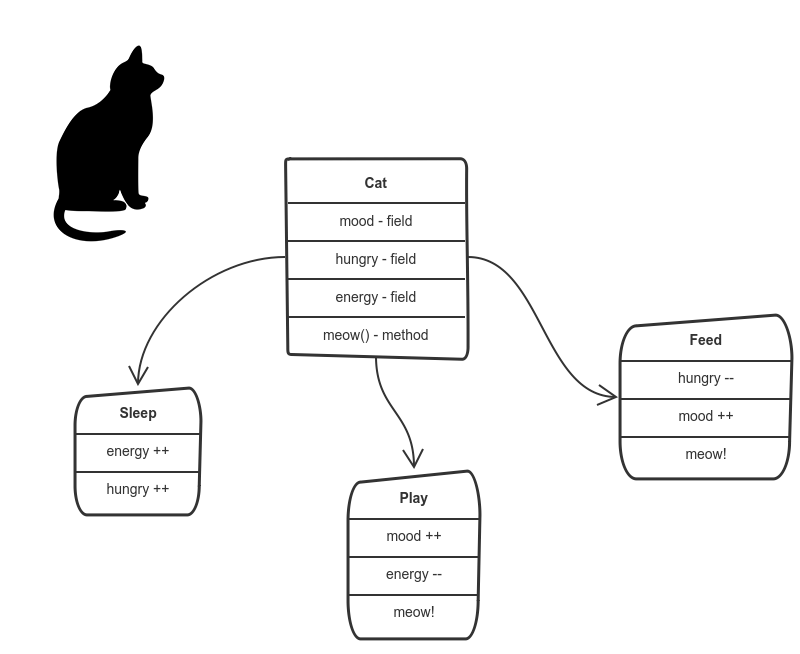
\includegraphics[width=.95\textwidth]{figures/classes.png}
    \caption[A visualization of a Cat Class including the Fields and Methods]{A visualization of a Cat Class including the Fields and Methods  \cite{classes}}
    \label{fig:classes}
\end{figure}

SINATRA is based in object oriented programming. Object oriented programming is a method of developing which utilizes `objects' that can be given variable characteristics. This allows a developer to create an object for a type of item in their program and then create many of those objects each with varying characteristics. It opens the door to functions being associated with various objects and those objects containing an idea of `self' in referring to the characteristics of that particular instance of the object. A simple version of a class can be seen in Figure \ref{fig:classes}. \par

\indent This method is particularity helpful in DSMC simulations. There are two large data structures which must be tracked: the mesh and the particles. A class structure fits right into that gap. Refer to Galvez's Thesis to see the exact breakdown of data structures used in SINATRA \cite{Galvez2018a}. \par

\subsection{Octree Mesh}
\label{sec:octree}

Another important feature of SINATRA is the octree mesh. Octree is a tree method of storing data, where each parent item has 8 children. An octree mesh has two main benefits; it is a well known data structure which is well documented and serves as a mesh refinement algorithm. A small example of the octree structure and it's refinement capability can be seen in Figure \ref{fig:octree}. \par


\begin{figure}
    \centering
    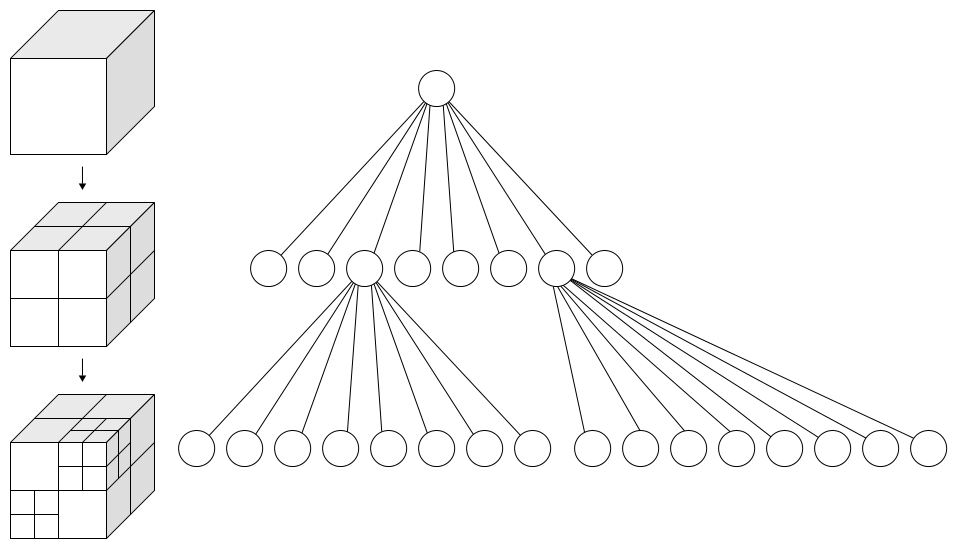
\includegraphics[width=.7\textwidth]{figures/octree.png}
    \caption[A demonstration of an octree mesh and it's data structure]{A demonstration of an octree mesh and it's data structure  \cite{octree}}
    \label{fig:octree}
\end{figure}


\indent An octree mesh is built from a cube domain, which is cut into 8 initial cells. Then, depending on user settings, more refinement is made until the mesh is well generated for the simulation case. If the simulation wants to show a curved surface, the cells are refined near the surface until the mesh is a good approximation of the object. Optimal mesh settings are on a simulation to simulation basis and are a largely a user controlled portion of CFD analysis. However, a discussion on automatic mesh generation and adaptation can be found in Section \ref{sec:auto_mesh}. The important advantage of octree meshes for DSMC is that when a particle moves out of a cell, it is less computationally intensive to find into which cell it moved compared to more primitive algorithms. The system can move up one level to the original cell's parent and then search all of that parents children. This speeds up the linking phase of DSMC. \par



\subsection{Models Implemented}
\label{sec:models}

There are various ways to physically model particles and domains. A good CFD program will include multiple options for a simulation so the analyst can test different types to see which works best for their simulation case. Therefore, multiple models for boundaries, particle spheres, and collision schemes have been built into SINATRA by Alliston and Galvez \cite{Galvez2018a} \cite{mac_thesis}. The different types can be seen below. It is also important to note, these models have been built specifically for DSMC, taking into account the `super-particles' and statistical dependency. 


\begin{itemize}
    \item \textbf{Boundary Types} \\
    These define the boundary conditions of the walls of the domain.
    \begin{itemize}
        \item \textit{Inflow} \\
        This wall allows particles to be inserted into the domain through the inject particles algorithm.
        \item \textit{Outflow} \\
        The wall allows particles to leave the domain if they cross this boundary.
        \item \textit{Spectral}\\
        This wall is similar to a symmetry plane, the particles are reflected off this wall spectrally.
        \item \textit{Diffuse}\\
        This wall has particles collide with the wall as if there was a user defined imaginary gas on the other side of the wall.
        \item \textit{Periodic} \\
        This wall takes the particle which crosses it and injects it in the same place and position on the other periodic wall, allowing for cyclic simulations.
    \end{itemize}
    
    \item \textbf{Sphere Models}\\
    When modeling particles, it is important to have a model of the electron sphere around the particle and it's effective radius.
    \begin{itemize}
        \item \textit{Hard Sphere Model}\\
        This model gives each particle a set radius and cross section.
        \item \textit{Variable Hard Sphere Model}\\
        This model sets the hard sphere depending on transitional energy.
        \item \textit{Variable Soft Sphere Model}\\
        This model takes into account the collision partner particle when determining the cross section.
    \end{itemize}
    
    
    \item \textbf{Collision Schemes} \\
    There are many different ways to choose particles for collisions and to simulate those collisions. Note - it is also possible in SINATRA to turn off collisions.
    \begin{itemize}
        \item \textit{Discrete Sub-Cell}\\
        This method cuts each cell into smaller sub-cells, then chooses particles from the sub cell to collide using an accept reject method. 
        \item \textit{Nearest Neighbor Scheme}\\
        This method checks the distance between every particle in the cell and chooses the closest particles as the collision partner.
        \item \textit{Trajectory Scheme}\\
        This method takes the trajectory of the particle in question, creates a virtual sub-cell from it's projected position, and then chooses a collision partner from that. 
    \end{itemize}
\end{itemize}


\subsection{Output Methods}
\label{sec:output}

Finally, an important part of a DSMC simulation is outputting the properties of the flow. SINATRA has three main methods for outputting information. The first is the simple timestep file. This file is appended to after SINATRA completes each timestep. This allows the simulation to be tracked as it is being run in the background. The next method is the main macro-properties sampler. It goes through all the sample cells, which can either be the lowest or second lowest level of cells and performs two loops. First it looks at all the particles in that cell and sums their properties, then it goes through all the species and calculates the various averages and data for which the specific output case calls. These values are output in a TecPlot\textsuperscript{TM} format and can be adjusted to be printed out every time step or every few steps. The final output method prints out each particle location and velocity. This creates a strong debugging tool to understand exactly what is happening in the flow. 